\documentclass{article}
\usepackage{graphicx}
\usepackage[hidelinks]{hyperref}
\usepackage{float}
\usepackage[utf8]{inputenc}
\usepackage[spanish]{babel}
\usepackage{csquotes}
\usepackage{listings}
\usepackage[a4paper, left=3cm, right=2.5cm, top=3cm, bottom=3cm]{geometry}
\usepackage{fancyhdr}
\usepackage{lastpage}
\usepackage{minted}
\usepackage{tikz}
\usepackage{xcolor}
\usepackage[bottom]{footmisc}
\usepackage{booktabs}
\usepackage{pdflscape}
\usepackage{adjustbox}
\usepackage[backend=biber, style=numeric]{biblatex}
\usepackage{bookmark}
\usepackage[nottoc]{tocbibind}

% Configuración de la bibliografía
\addbibresource{references.bib}

% Definición de nuevos comandos
\newcommand{\mail}[2]{\href{mailto:#1}{#2}}
\definecolor{mygreen}{RGB}{124, 180, 76}
\definecolor{mycyan}{RGB}{100, 124, 204}

\pagestyle{fancy}
\fancyhf{}
 
\fancyfoot[R]{Página \thepage\ de \pageref{LastPage}}

% Definir un estilo para las páginas landscape con "Página X de Y" alineado a la derecha sin negrita
\fancypagestyle{landscape}{
  \fancyhf{}  % Limpiar encabezado y pie de página
  \fancyfoot{%
    \tikz[remember picture,overlay]
      \node[outer sep=2cm,above,rotate=90] at (current page.east) {Página \thepage\ de \pageref{LastPage}};}
}

\setlength{\parindent}{0pt}

\renewcommand{\headrulewidth}{0pt}
\renewcommand{\footrulewidth}{0pt}

\lstset{
    basicstyle=\ttfamily, % Estilo monoespaciado para el código
    breaklines=true,      % Romper líneas largas automáticamente
    breakatwhitespace=true, % Romper líneas largas en espacios
}

\graphicspath{{images/}}

\definecolor{highlightcolor}{rgb}{1.0, 0.76, 0.0}
\definecolor{bgcolor}{rgb}{0.95, 0.95, 0.95}

% Definición de la portada del documento
\title{
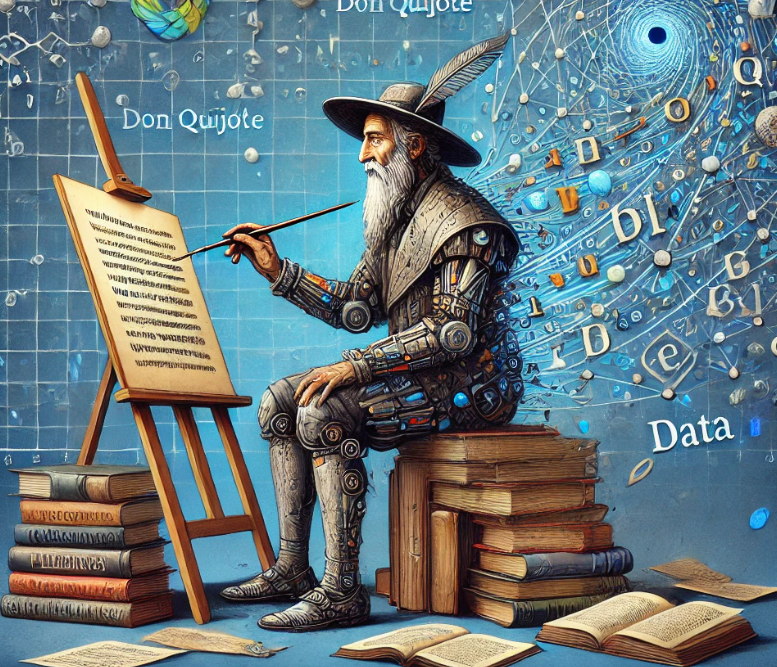
\includegraphics[scale=0.5]{don_quijote_generativo.png} \\
\vspace{2em}
\textbf{Deep Learning} \\ \rule{0.8\textwidth}{0.5pt} \\ \large \textbf{Programación de Bases de Datos}}
\author{Daniel Torres Galindo \thanks{dtorrescb@alumnos.unex.es} \and Daniel Sánchez Parra \thanks{dsanchezfe@alumnos.unex.es}}
\date{\today}

% Cambiar el formato de los números de las notas a pie de página
\makeatletter
\let\@fnsymbol\@arabic
\makeatother

\begin{document}

\maketitle

\thispagestyle{empty}

\begin{figure}[H]
    \centering
    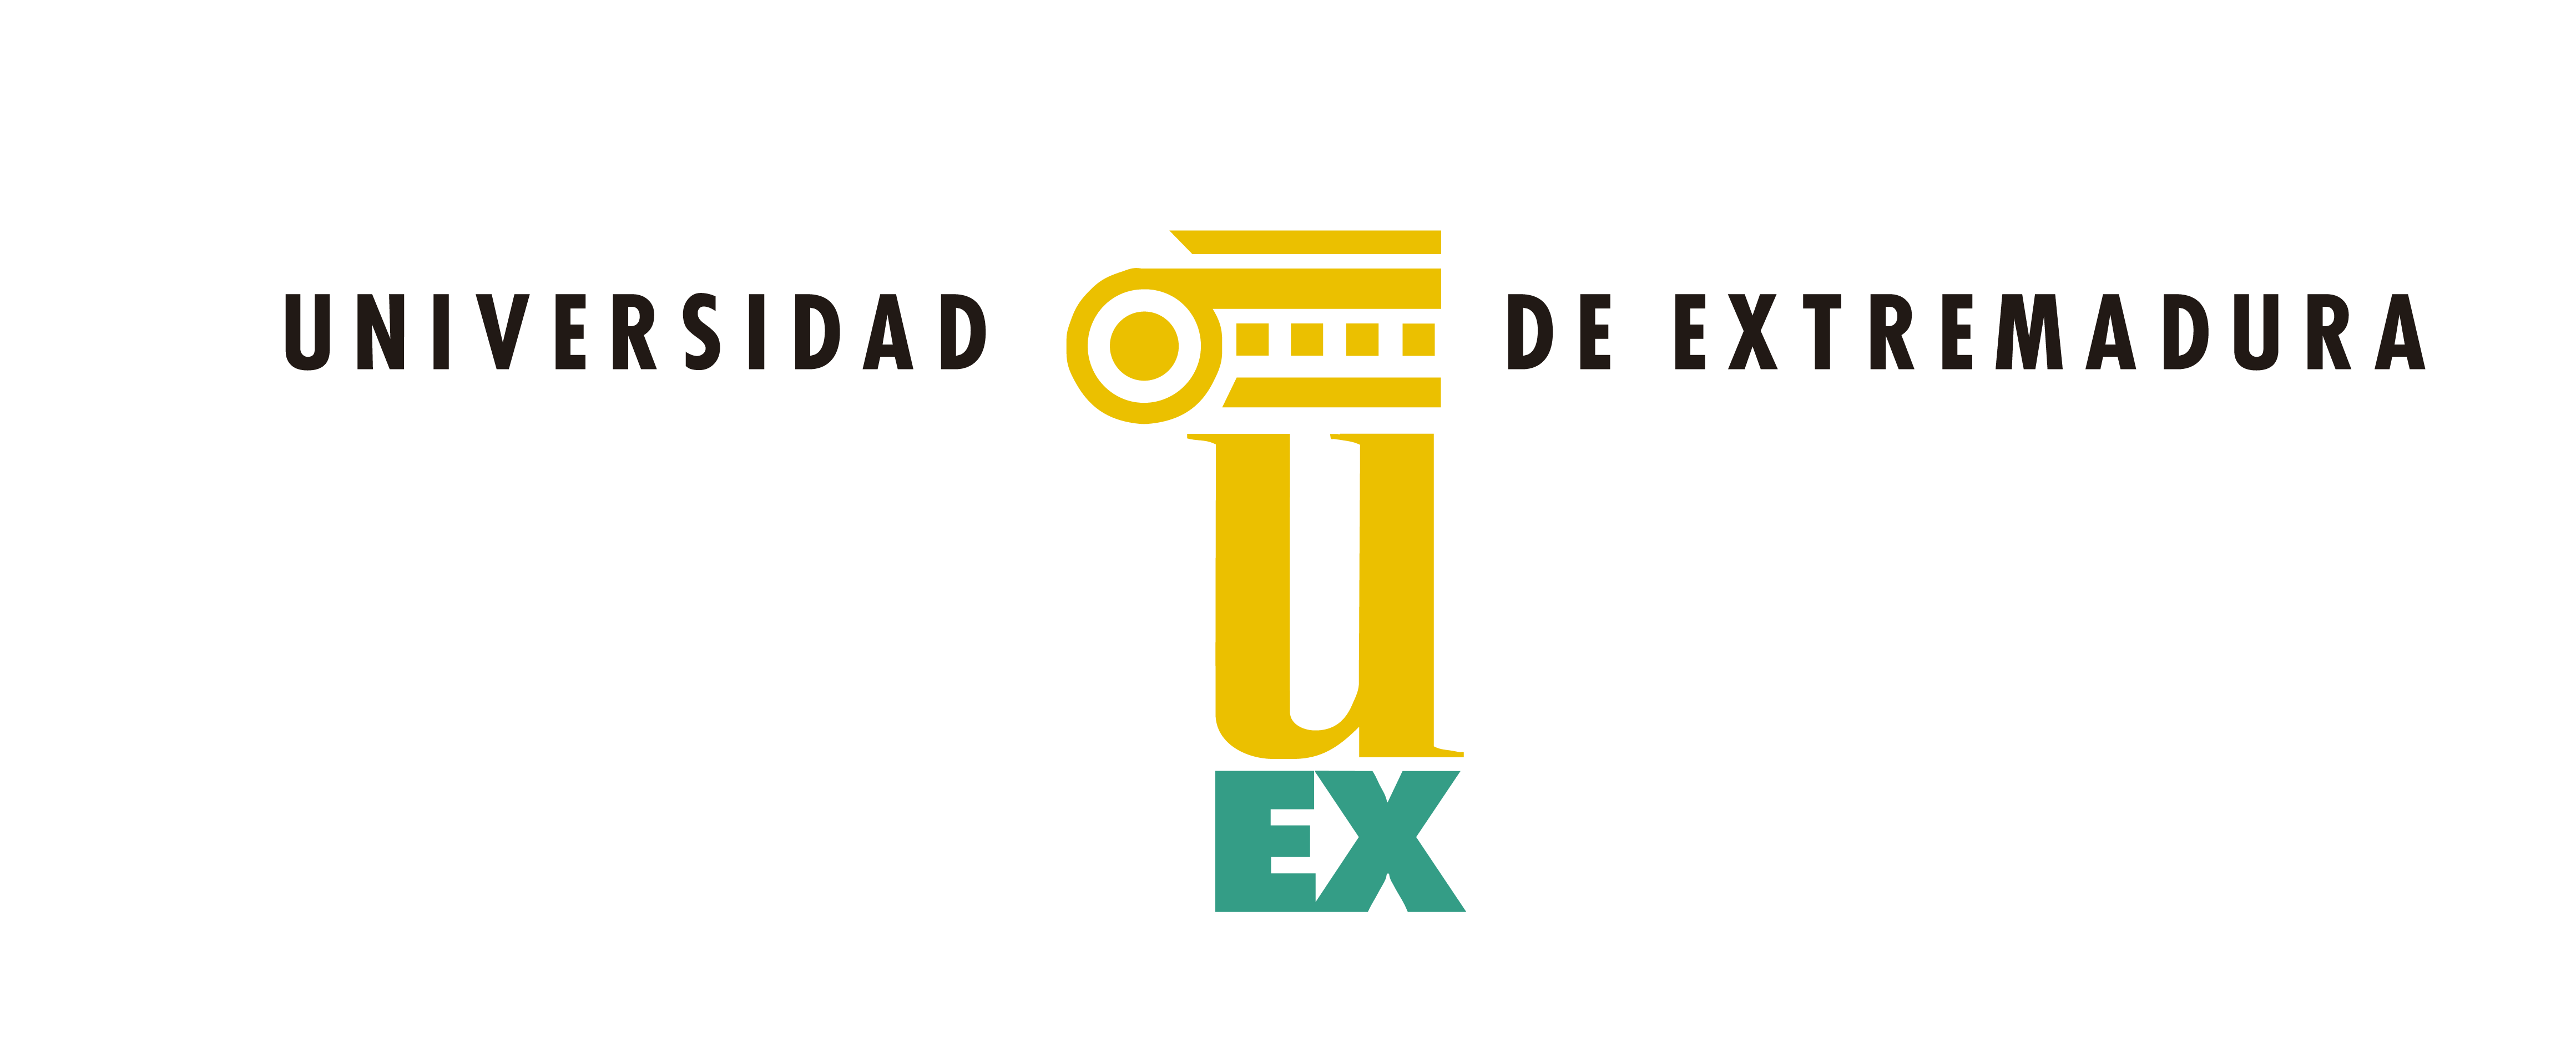
\includegraphics[width=0.7\textwidth]{logo-uex.png}
\end{figure}

% Línea de pie de página de la portada
\renewcommand{\footnoterule}{
    \vspace{1em}
    \hrule width \linewidth height 0.5pt
    \vspace{0.5em}
}

\newpage

\tableofcontents

\newpage

\section{Introducción}
\subsection{Contexto y objetivo del proyecto}
En un mundo donde el procesamiento del lenguaje natural (NLP, por sus siglas en inglés) está revolucionando la forma en que interactuamos con la tecnología, el desarrollo de modelos capaces de generar texto de manera autónoma se ha convertido en un tema clave.
Desde asistentes virtuales como Siri y Alexa hasta herramientas avanzadas de escritura asistida, los sistemas de generación de texto están transformando industrias enteras. \\

El presente proyecto busca explorar esta tecnología utilizando una obra literaria clásica, \textbf{Don Quijote de la Mancha}, como conjunto de datos base.
A través del uso de Redes Neuronales Recurrentes (RNN), especialmente diseñadas para manejar datos secuenciales, pretendemos imitar el estilo de escritura de Miguel de Cervantes, generando texto carácter por carácter.
Este enfoque no solo pone a prueba la capacidad del modelo para capturar dependencias complejas en el lenguaje, sino que también muestra cómo las técnicas de Deep Learning pueden aplicarse en dominios creativos. \\

\subsection{Objetivos específicos}

\begin{itemize}
    \item \textbf{Preparación de Datos}: Descargar, preprocesar y tokenizar el texto de \emph{Don Quijote de la Mancha} para convertirlo en un formato adecuado para entrenamiento de modelos.
    \item \textbf{Diseño del Modelo}: Construir una arquitectura basada en RNN que incluya capas de embeddings, LSTM, y una capa de salida para predicción carácter por carácter.
    \item \textbf{Entrenamiento}:
    \begin{itemize}
        \item Ajustar hiperparámetros como tamaño del batch, número de épocas y función de pérdida.
        \item Implementar un proceso de entrenamiento eficiente que permita capturar las dependencias a largo plazo presentes en el texto.
    \end{itemize}
    \item \textbf{Generación de Texto}:
    \begin{itemize}
        \item Utilizar el modelo entrenado para generar texto de forma iterativa, ajustando la temperatura para variar la creatividad en las predicciones.
    \end{itemize}
    \item \textbf{Evaluación}:
    \begin{itemize}
        \item Analizar los textos generados, comparándolos con el estilo literario del texto original.
        \item Evaluar la coherencia, fluidez y calidad del texto generado.
    \end{itemize}
\end{itemize}

\newpage

\section{Marco Teórico}
\subsection{Introducción al Deep Learning}
\subsubsection{¿Qué es el Deep Learning?}
El deep learning es un subconjunto del machine learning \cite{ibm-ml} que utiliza redes neuronales \cite{ibm-nn} multicapa, llamadas redes neuronales profundas, para simular el complejo poder de toma de decisiones del cerebro humano. Algunas formas de deep learning impulsan la mayoría de las aplicaciones de inteligencia artificial \cite{ibm-ia} (IA) en nuestra vida actual. \\

La principal diferencia entre el deep learning y el machine learning es la estructura de la arquitectura de red neuronal subyacente. Los modelos tradicionales de machine learning \cite{ibm-ml-types} ``no profundos'' utilizan redes neuronales simples con una o dos capas computacionales. Los modelos de deep learning utilizan tres o más capas, pero normalmente cientos o miles de capas, para entrenar los modelos. \\

\begin{figure}[H]
    \centering
    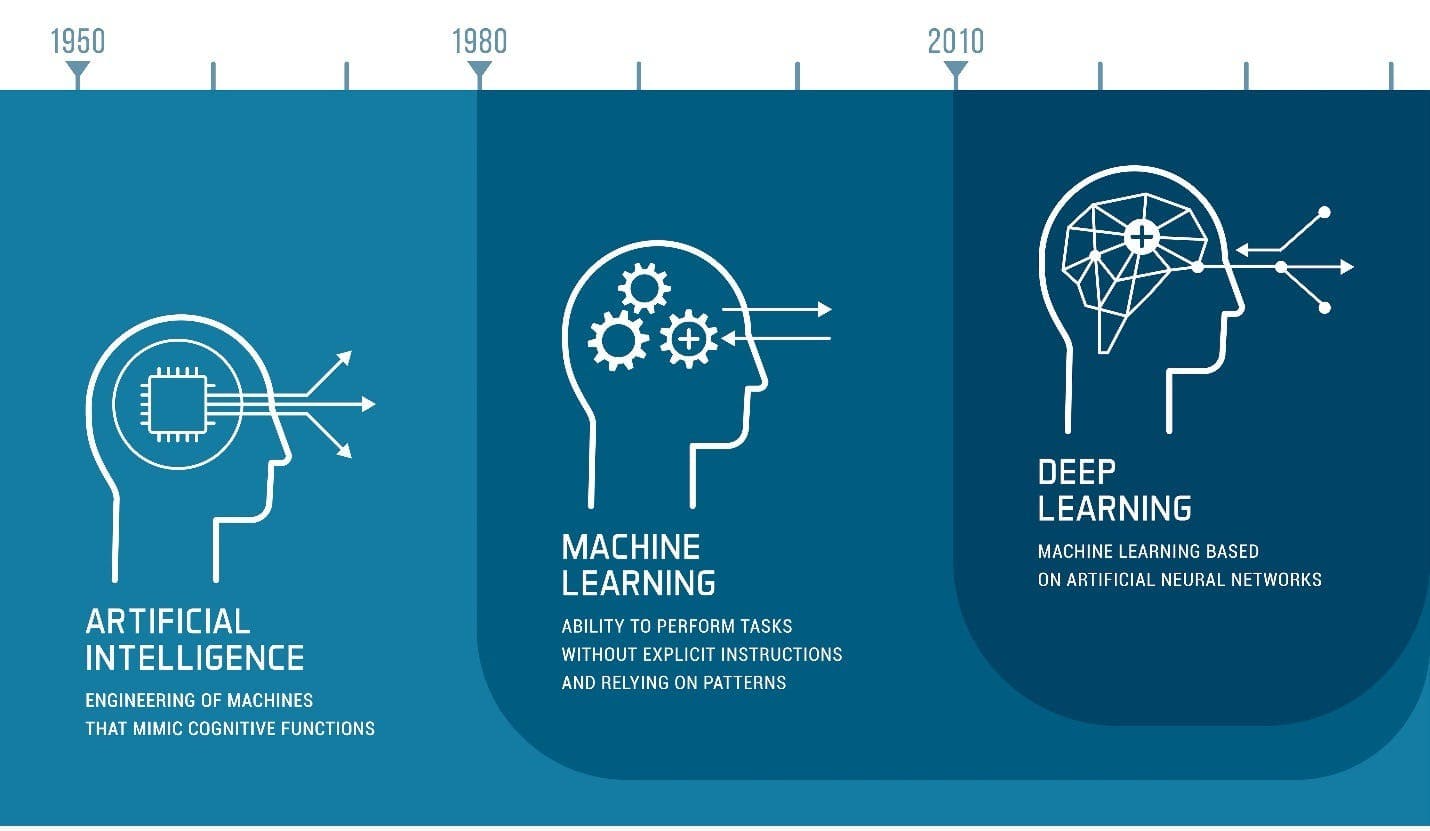
\includegraphics[scale=0.2]{history.png}
    \caption{Cronograma sobre el avance de la Inteligencia Artificial. \cite{tjk2024deep}}
\end{figure}

Mientras que los modelos de aprendizaje supervisado requieren datos de entrada estructurados y etiquetados para obtener resultados precisos, los modelos de deep learning pueden utilizar el aprendizaje no supervisado. Con el aprendizaje no supervisado, los modelos de deep learning pueden extraer las características, los rasgos y las relaciones que necesitan para obtener resultados precisos a partir de datos brutos y no estructurados. Además, estos modelos pueden incluso evaluar y refinar sus resultados para aumentar la precisión. \\

\begin{figure}[H]
    \centering
    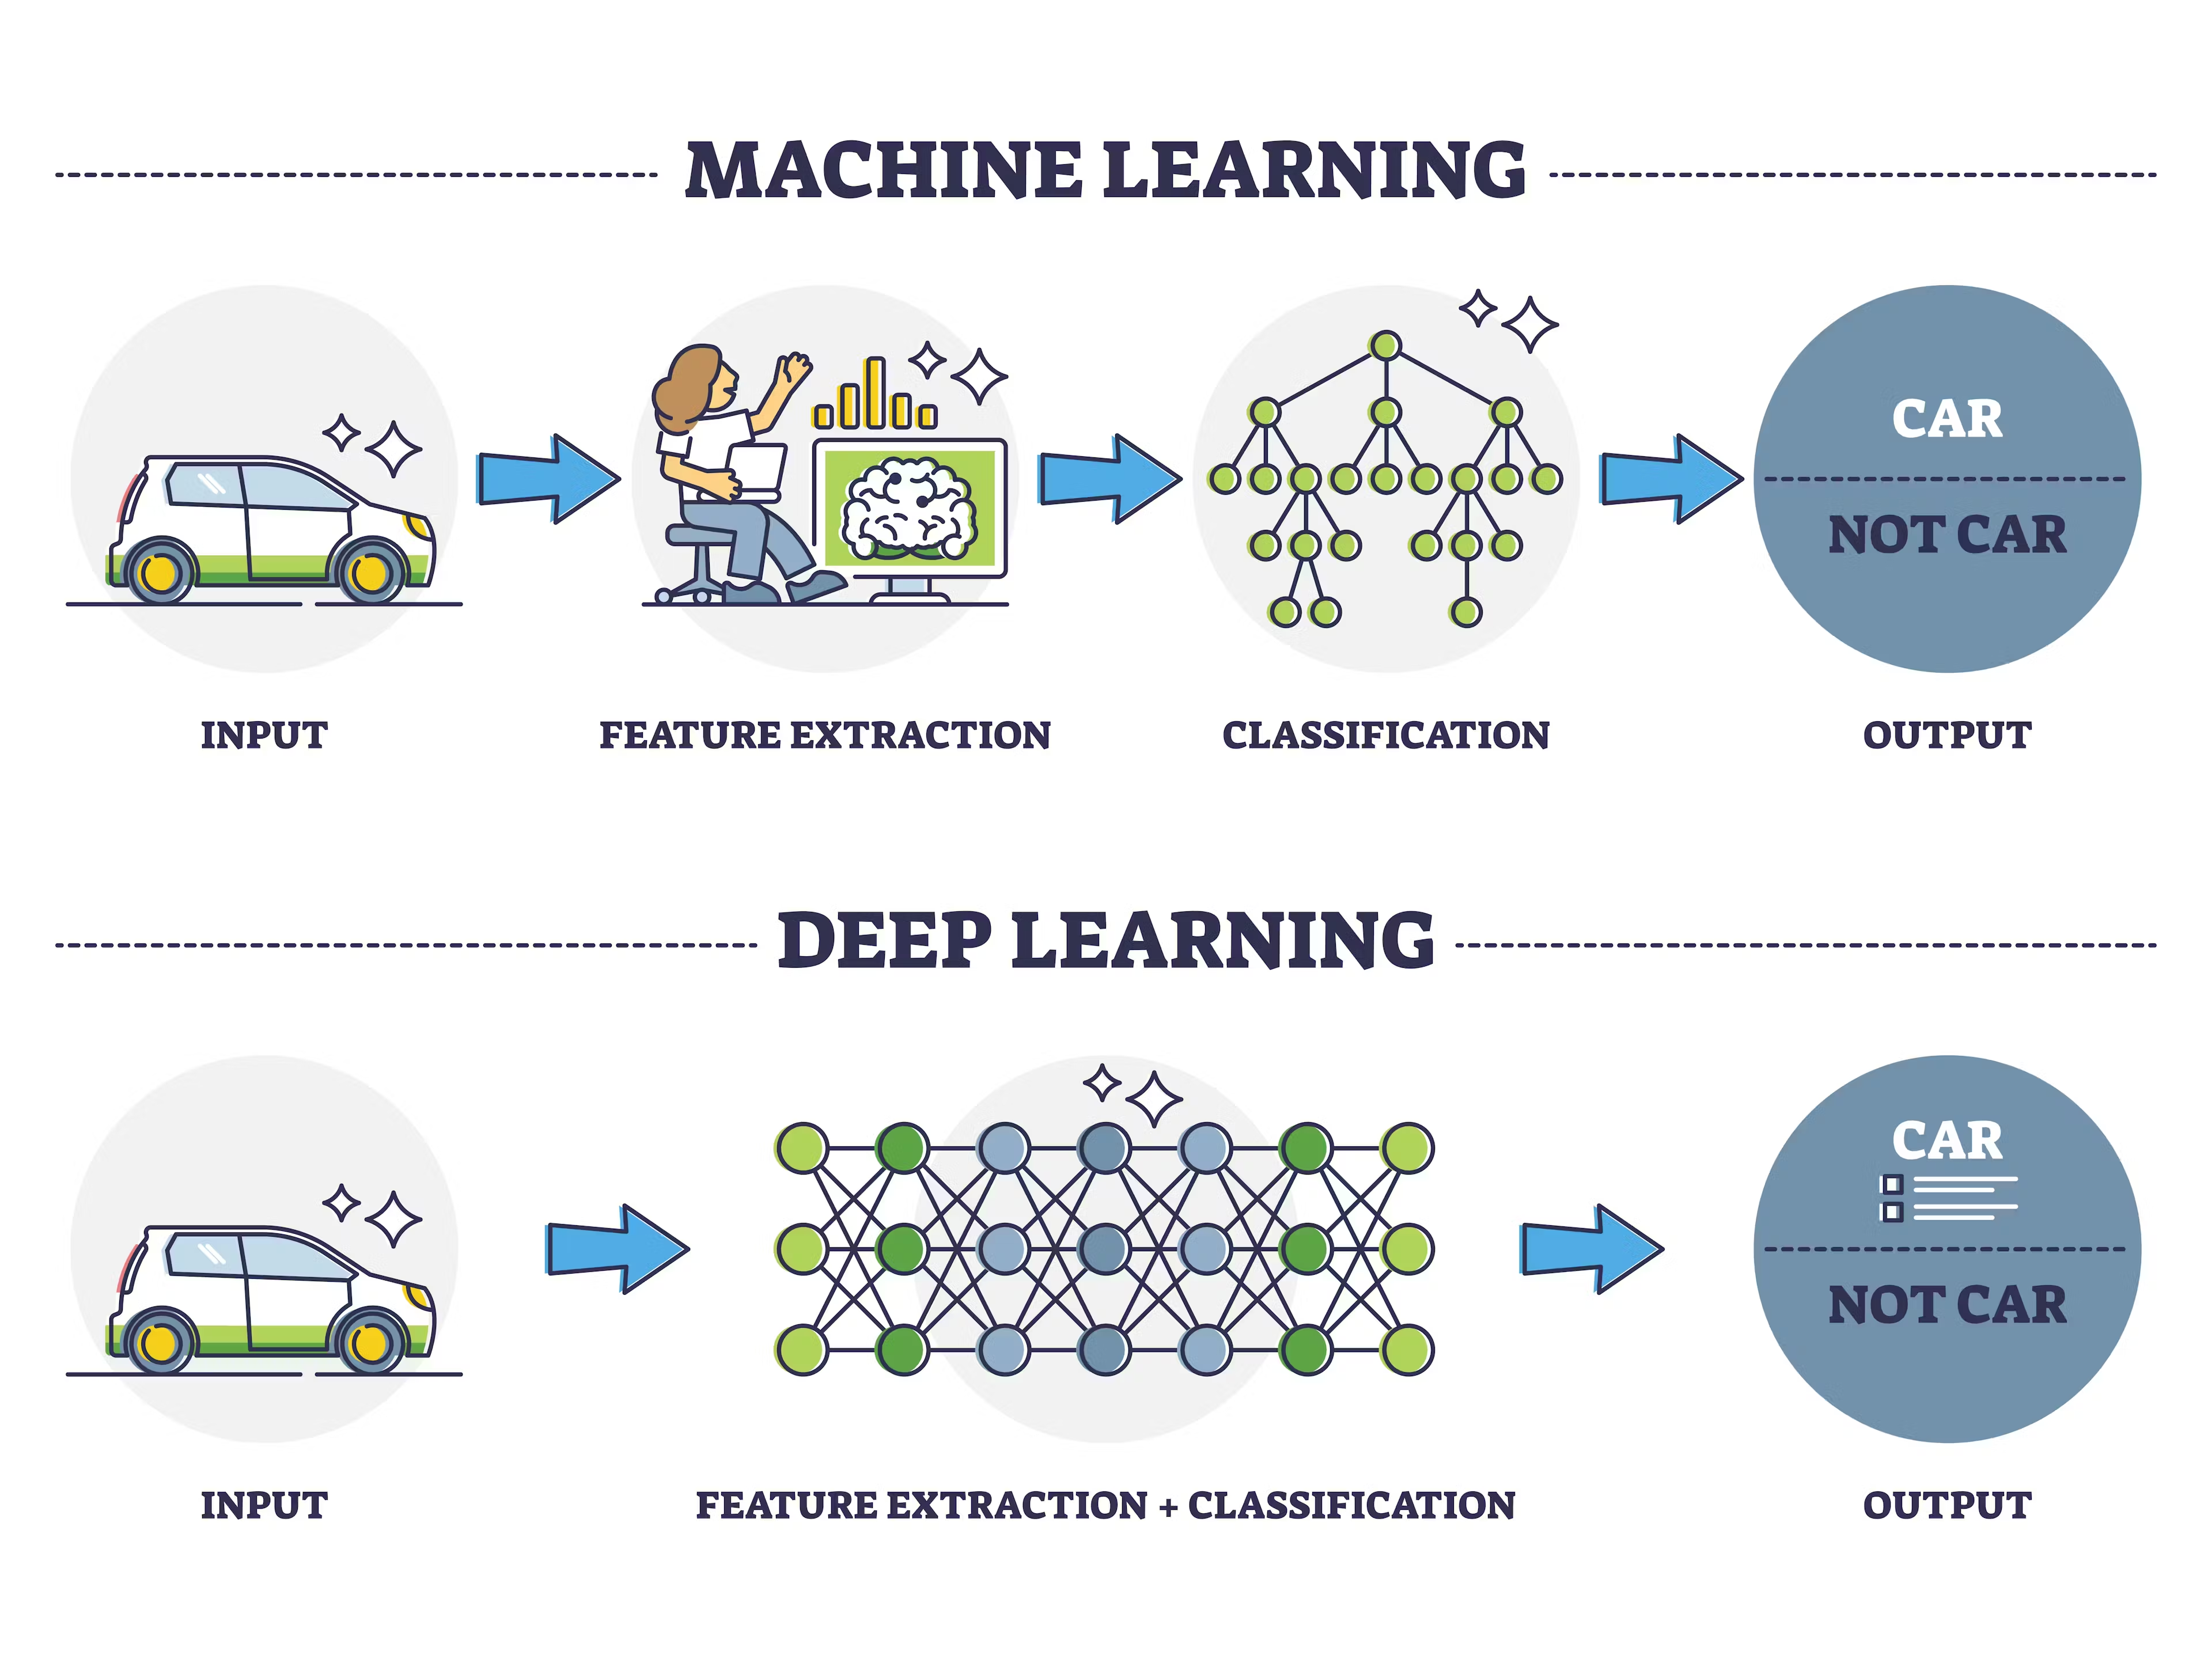
\includegraphics[scale=0.075]{mlvsdp.png}
    \caption{Machine Learning vs Deep Learning.}
\end{figure}

El deep learning es un aspecto de la ciencia de datos que impulsa muchas aplicaciones y servicios que mejoran la automatización, realizando tareas analíticas y físicas sin intervención humana. Esto permite muchos productos y servicios cotidianos, como asistentes digitales, controles remotos de TV habilitados para voz, detección de fraudes con tarjetas de crédito, automóviles autónomos e IA generativa. \\

\newpage

\subsubsection{¿Cómo funciona el Deep Learning?}
Las redes neuronales, o redes neuronales artificiales, intentan imitar el cerebro humano a través de una combinación de entradas de datos, ponderaciones y sesgos, todos actuando como neuronas de silicio. Estos elementos trabajan juntos para reconocer, clasificar y describir con precisión los objetos dentro de los datos. \\

Las redes neuronales profundas se componen de varias capas de nodos interconectados, cada una de las cuales se basa en la capa anterior para refinar y optimizar la predicción o la categorización. Esta progresión de cálculos a través de la red se denomina propagación hacia adelante. Las capas de entrada y salida de una red neuronal profunda se denominan capas visibles . La capa de entrada es donde el modelo de deep learning ingiere los datos para su procesamiento, y la capa de salida es donde se realiza la predicción o clasificación final. \\

\begin{figure}[H]
    \centering
    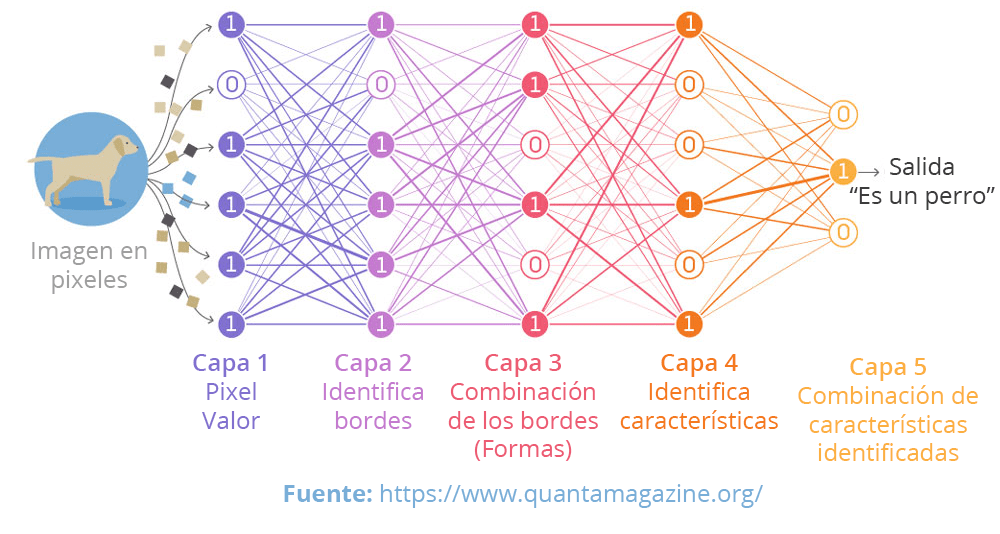
\includegraphics[scale=0.3]{layers.png}
    \caption{Red Neuronal.}
\end{figure}

El deep learning requiere una enorme cantidad de potencia informática. Las unidades de procesamiento gráfico (GPU) de alto rendimiento son ideales porque pueden manejar un gran volumen de cálculos en varios núcleos con memoria copiosa disponible. El cloud computing distribuida también podría resultar útil. Este nivel de potencia de cómputo es necesario para entrenar algoritmos profundos a través del deep learning. Sin embargo, gestionar varias GPU en las instalaciones puede generar una gran demanda de recursos internos y su escalamiento es increíblemente caro. Para los requisitos de software, la mayoría de las aplicaciones de deep learning están codificadas con uno de estos tres marcos de aprendizaje: JAX, PyTorch o TensorFlow. \\

\newpage

\subsection{Redes Neuronales Recurrentes (RNN)}
\subsubsection{¿Qué son las RNN?}
Una red neuronal recurrente, o (RNN), es una red neuronal \cite{ibm-nn} profunda entrenada con datos secuenciales o de series temporales para crear un modelo de machine learning \cite{ibm-ml} que pueda hacer predicciones secuenciales o conclusiones basadas en entradas secuenciales. \\

Una (RNN) podría utilizarse para predecir los niveles diarios de inundación basándose en los datos diarios anteriores sobre inundaciones, mareas y meteorología.
Pero las (RNN) también se pueden utilizar para resolver problemas ordinales o temporales, como la traducción de idiomas, el procesamiento del lenguaje natural (PLN) \cite{ibm-pln}, el reconocimiento de voz \cite{ibm-sr} y el subtitulado de imágenes.
Las (RNN) se incorporan a aplicaciones populares como Siri, búsqueda por voz y Google Translate.

\subsubsection{Funcionamiento de las RNN}
Al igual que [las redes neuronales convolucionales CNN \cite{ibm-cnn}, las redes neuronales recurrentes utilizan datos de entrenamiento para aprender.
Se distinguen por su ``memoria'', ya que toman la información de las entradas anteriores para influir en la entrada y la salida actuales.
Aunque las redes neuronales profundas tradicionales asumen que las entradas y las salidas son independientes entre sí, la salida de los (RNN) depende de los elementos anteriores de la secuencia.
Mientras que las redes neuronales profundas tradicionales asumen que las entradas y las salidas son independientes entre sí, la salida de las (RNN) depende de los elementos anteriores dentro de la secuencia. \\

Tomemos un modismo, como el inglés ``feeling under the weather'', que se utiliza comúnmente cuando alguien está enfermo, para ayudarnos en la explicación de las (RNN).
Para que el modismo tenga sentido, debe expresarse en ese orden específico.
En consecuencia, las redes recurrentes deben tener en cuenta la posición de cada palabra en el modismo y utilizan esa información para predecir la siguiente palabra de la secuencia.

\begin{figure}[H]
    \centering
    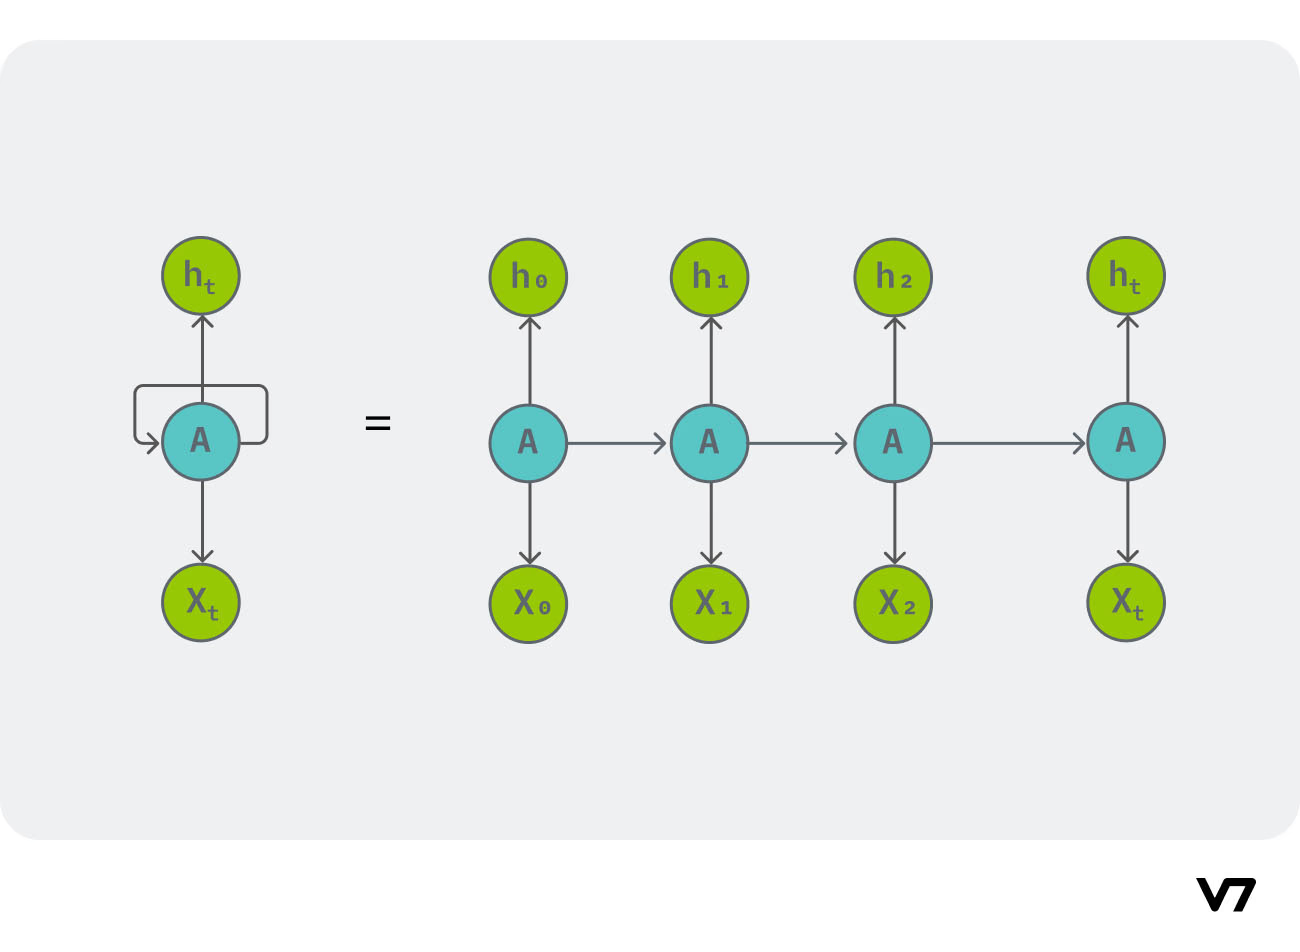
\includegraphics[scale=0.2]{secuencia.png}
    \caption{Secuencia y pesos en una RNN.}
\end{figure}

Otra característica distintiva de las redes recurrentes es que comparten parámetros en cada capa de la red.
Mientras que las redes feedforward tienen diferentes pesos en cada nodo, las redes neuronales recurrentes comparten el mismo parámetro de peso dentro de cada capa de la red.
Dicho esto, estos pesos todavía se ajustan a través de los procesos de retropropagación y descenso de gradiente para facilitar el aprendizaje por refuerzo.

\newpage

Las redes neuronales recurrentes aprovechan los algoritmos de retropropagación a través del tiempo (BPTT, por sus siglas en inglés) para determinar los gradientes, lo que difiere ligeramente de la retropropagación tradicional, ya que es específica de los datos secuenciales.
Los principios de la (BPTT) son los mismos que los de la retropropagación tradicional, en la que el modelo se entrena a sí mismo calculando los errores de su capa de salida a su capa de entrada.
Estos cálculos nos permiten ajustar y ajustar los parámetros del modelo adecuadamente.
(BPTT) difieren del enfoque tradicional en que estas suman errores en cada paso de tiempo mientras que las redes feedforward no necesitan sumar errores ya que no comparten parámetros a través de cada capa.

\begin{figure}[H]
    \centering
    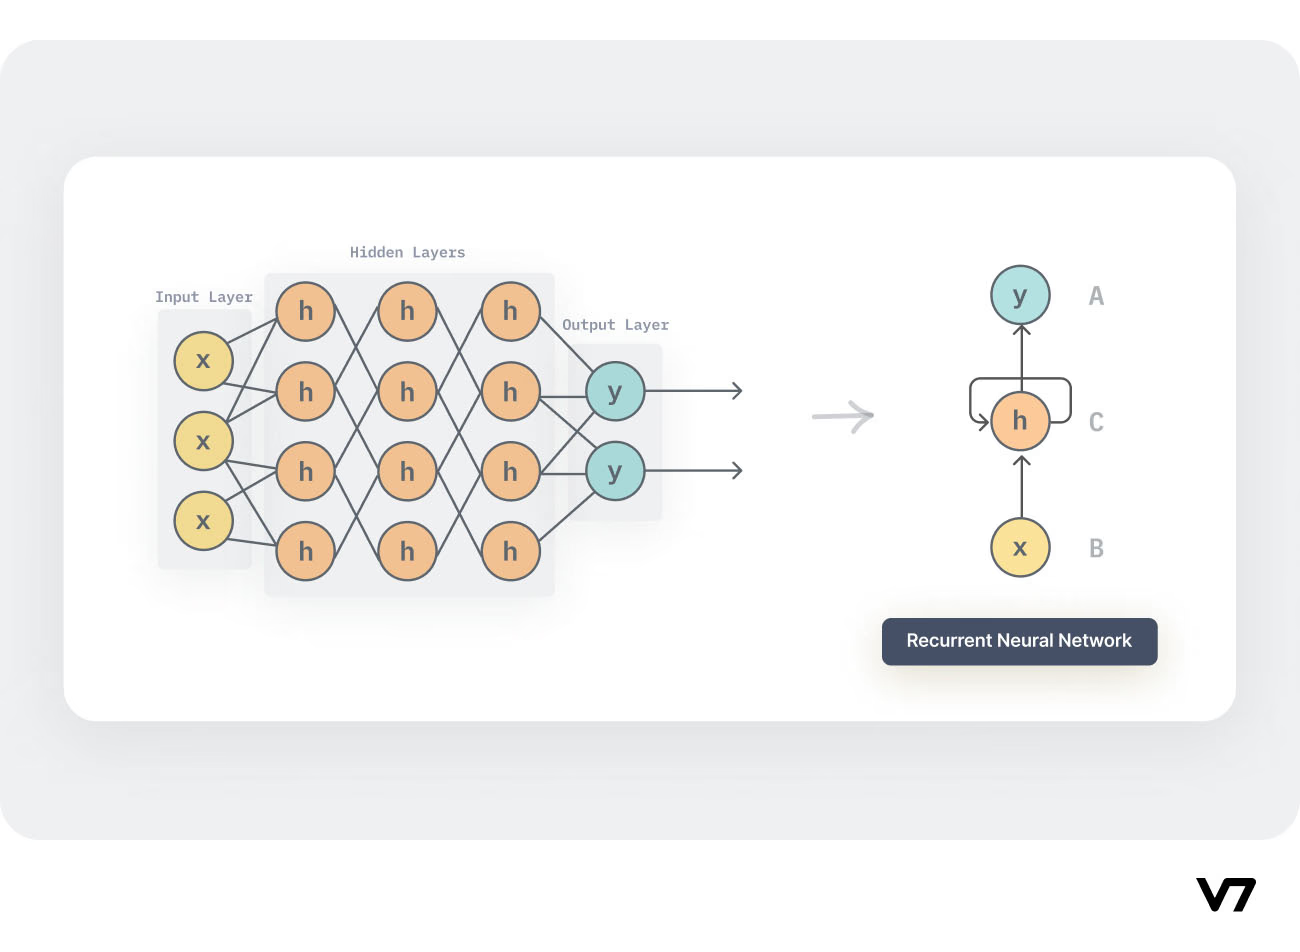
\includegraphics[scale=0.25]{capas.png}
    \caption{Capas en una red neuronal.}
\end{figure}

Durante este proceso, las (RNN) tienden a enfrentarse a dos problemas, conocidos como gradientes de explosión y gradientes de desaparición.
Estos problemas se definen por el tamaño del gradiente, que es la pendiente de la función de pérdida a lo largo de la curva de error.
Cuando el gradiente es demasiado pequeño, sigue haciéndose más pequeño, actualizando los parámetros de peso hasta que se vuelven insignificantes, es decir, cuando eso ocurre, el algoritmo ya no está aprendiendo.
La explosión de gradientes sucede cuando el gradiente es demasiado grande, lo que crea un modelo inestable.
En este caso, los pesos del modelo crecerán demasiado y, finalmente, se representarán como \textit{NaN}.
Una solución a estos problemas es reducir el número de capas ocultas de la red neuronal, lo que elimina parte de la complejidad de los modelos (RNN).

\begin{figure}[H]
    \centering
    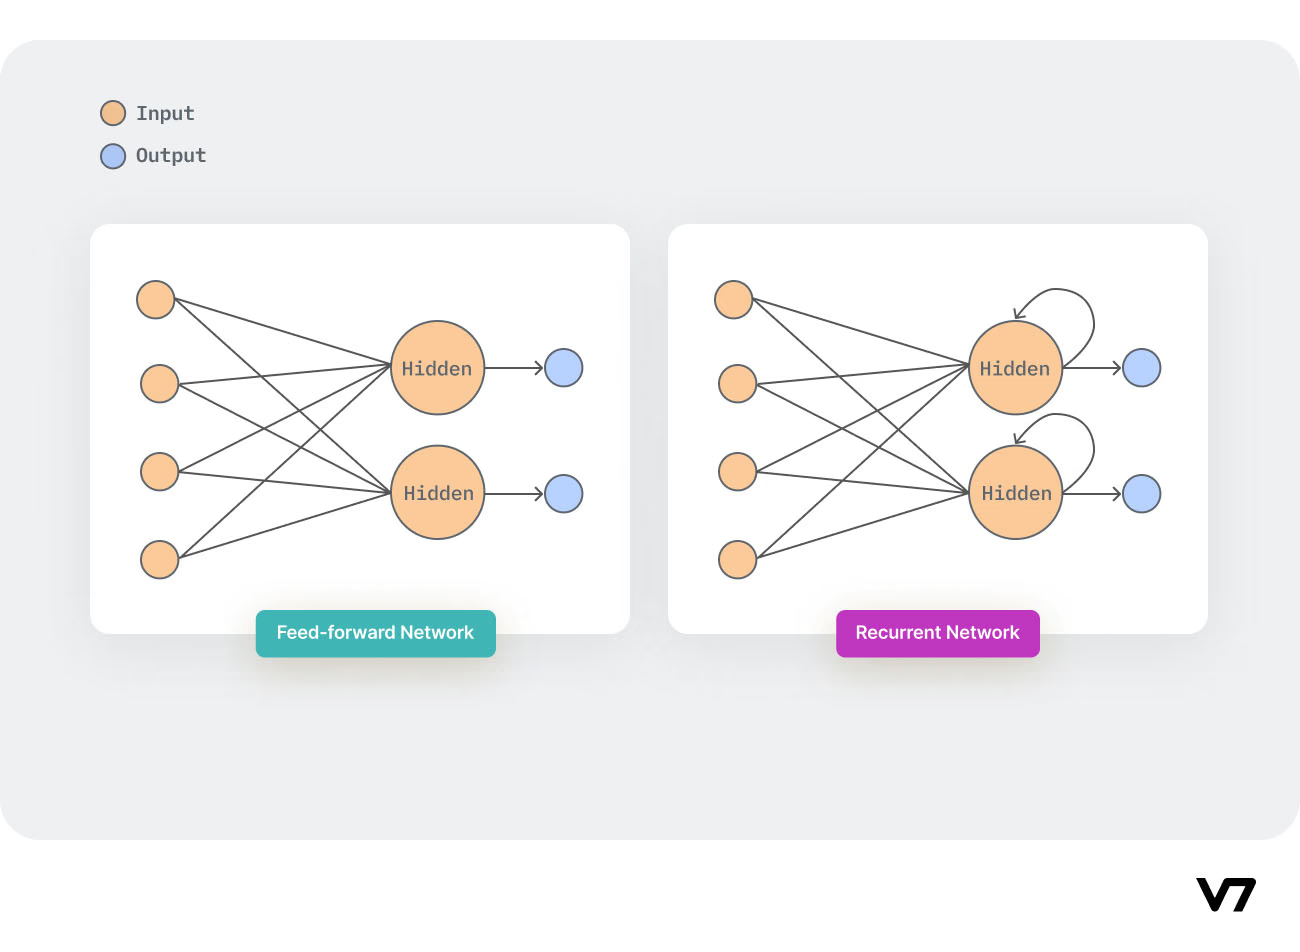
\includegraphics[scale=0.25]{ffrn.png}
    \caption{Feed-Forward Network vs Recurrent Network.}
\end{figure}

\newpage

\subsubsection{Tipos de RNN}
Las redes neuronales tradicionales tienen capas de entrada y salida independientes, lo que las hace inadecuadas para manejar datos secuenciales.
Las Redes Neuronales Recurrentes (RNN) se introdujeron para almacenar los resultados de salidas previas en una memoria interna.
Los cuatro tipos más comúnmente utilizados de Redes Neuronales Recurrentes son:

\begin{itemize}
    \item \textbf{One-To-One}: El tipo más simple de (RNN) es el One-to-One, que permite una sola entrada y una sola salida. Tiene tamaños de entrada y salida fijos, y actúa como una red neuronal estándar. Una de las aplicaciones del modelo One-to-One se encuentra en la clasificación de imágenes.
\end{itemize}

\begin{figure}[H]
    \centering
    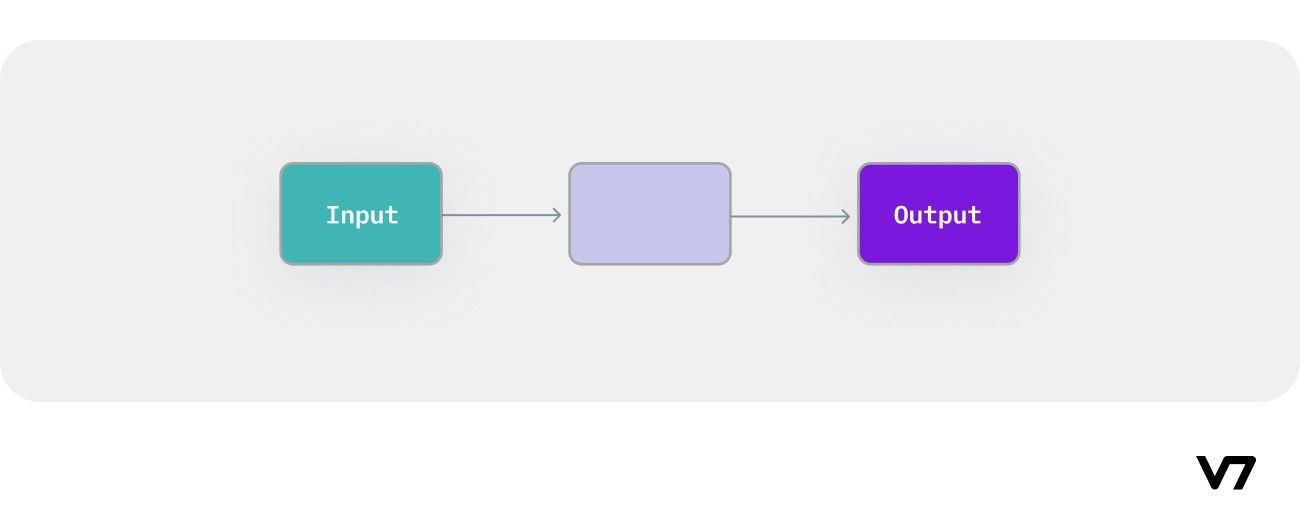
\includegraphics[scale=0.25]{oto.jpeg}
    \caption{One-To-One.}
\end{figure}

\begin{itemize}
    \item \textbf{One-To-Many}: El One-to-Many es un tipo de (RNN) que genera múltiples salidas a partir de una única entrada proporcionada al modelo. El tamaño de la entrada es fijo y produce una serie de datos como salida. Sus aplicaciones se encuentran en áreas como la generación de música y la generación de descripciones para imágenes (Image Captioning).
\end{itemize}

\begin{figure}[H]
    \centering
    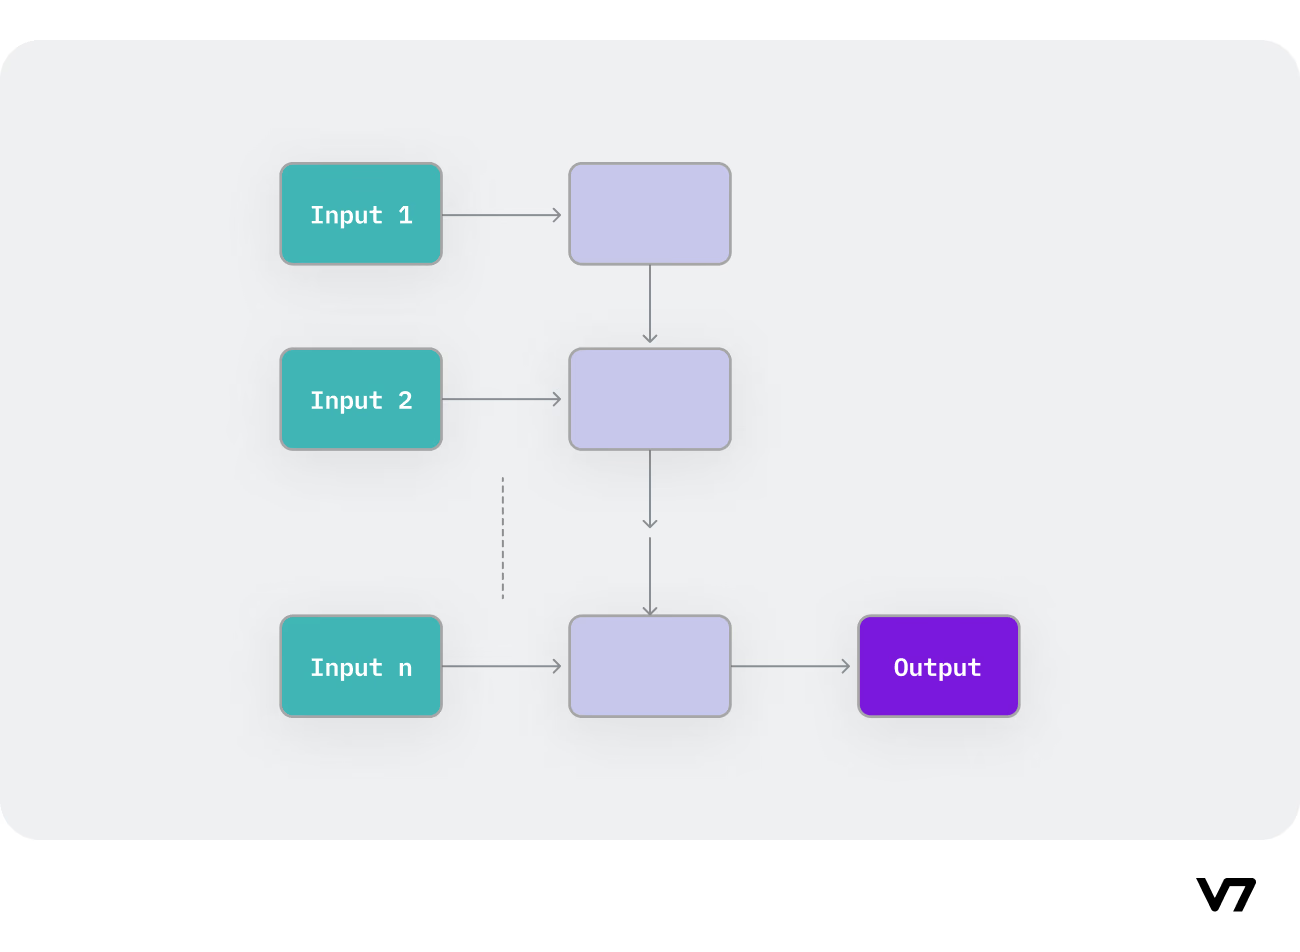
\includegraphics[scale=0.25]{mto.png}
    \caption{One-To-Many.}
\end{figure}

\newpage

\begin{itemize}
    \item \textbf{Many-To-Many}: es un tipo de RNN que se utiliza para generar una secuencia de datos de salida a partir de una secuencia de unidades de entrada. Este tipo se divide en las siguientes dos subcategorías:
    \begin{itemize}
        \item \textbf{Equal-Size}: En este caso, el tamaño de las capas de entrada y salida es exactamente el mismo.
    \end{itemize}
    \begin{figure}[H]
        \centering
        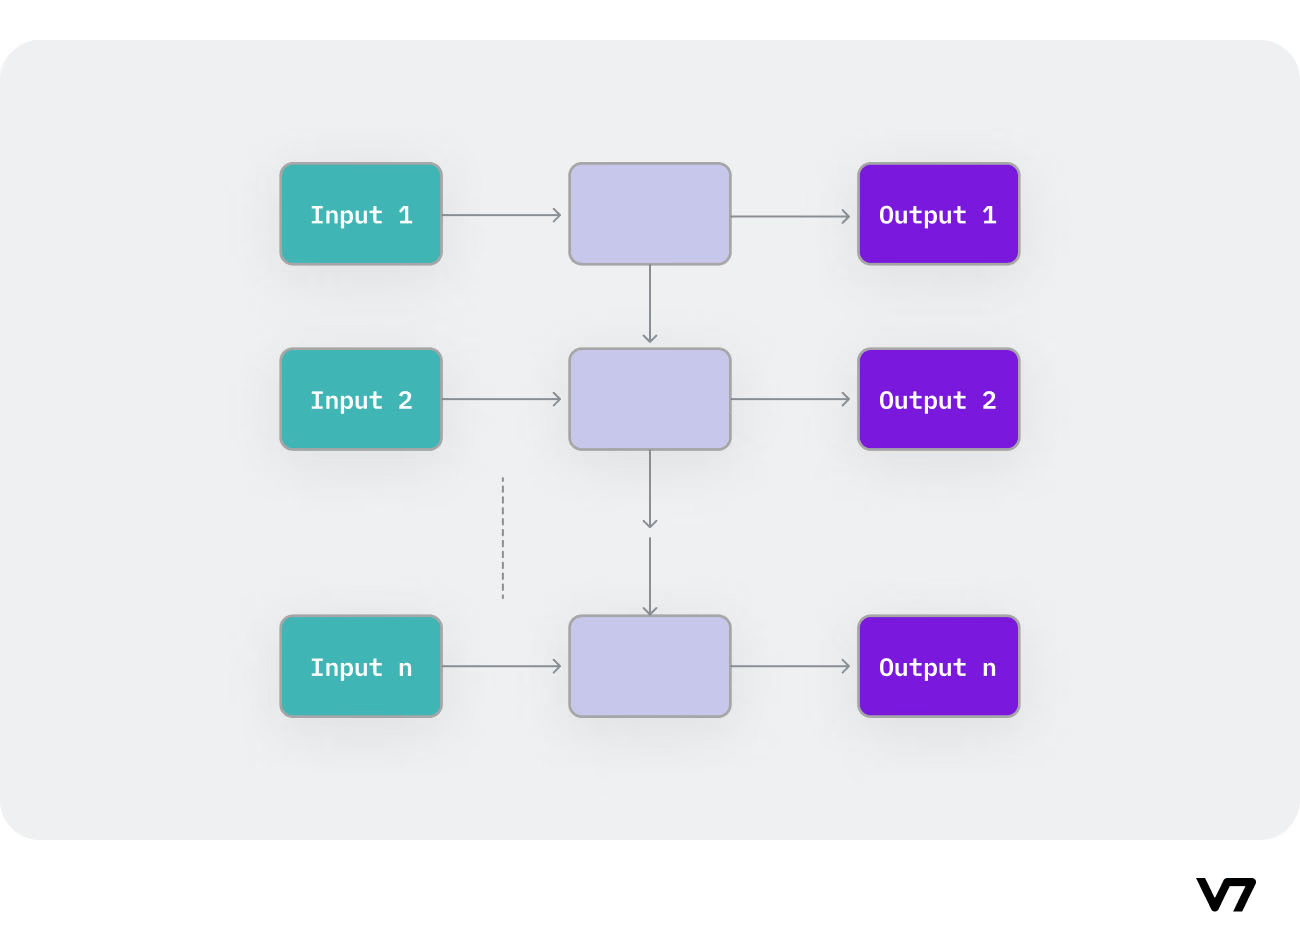
\includegraphics[scale=0.25]{mteq.png}
        \caption{Many-To-Many (Equal-Size).}
    \end{figure}
    \begin{itemize}
        \item \textbf{Unequal-Size}: En este caso, las entradas y salidas tienen un número diferente de unidades. Su aplicación se encuentra en la \textit{traducción automática} (Machine Translation).
    \end{itemize}
    \begin{figure}[H]
        \centering
        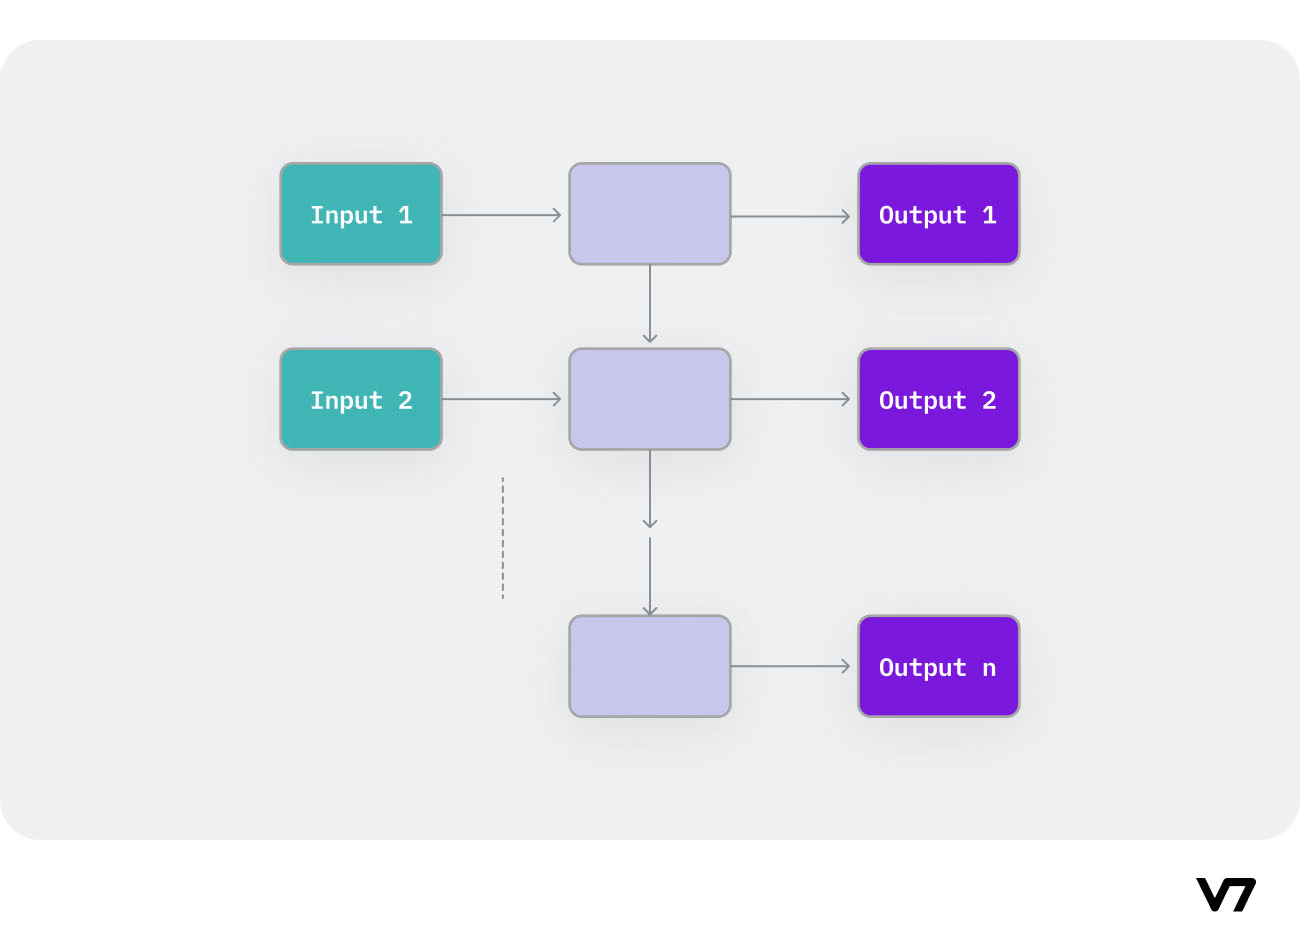
\includegraphics[scale=0.25]{mtun.png}
        \caption{Many-To-Many (Unequal-Size).}
    \end{figure}
\end{itemize}

\subsection{Arquitecturas RNN variantes}
\subsubsection{Redes neuronales recurrentes bidireccionales (BRNN)}
Mientras que en las RNN unidireccionales sólo se pueden extraer de entradas anteriores para hacer predicciones sobre el estado actual, las RNN bidireccionales, o BRNN, extraen datos futuros para mejorar la precisión de los mismos. Volviendo al ejemplo de ``feeling under the weather'', un modelo basado en una BRNN puede predecir mejor que la segunda palabra de esa frase es ``under'' si sabe que la última palabra de la secuencia es ``weather''.

\begin{figure}[H]
    \centering
    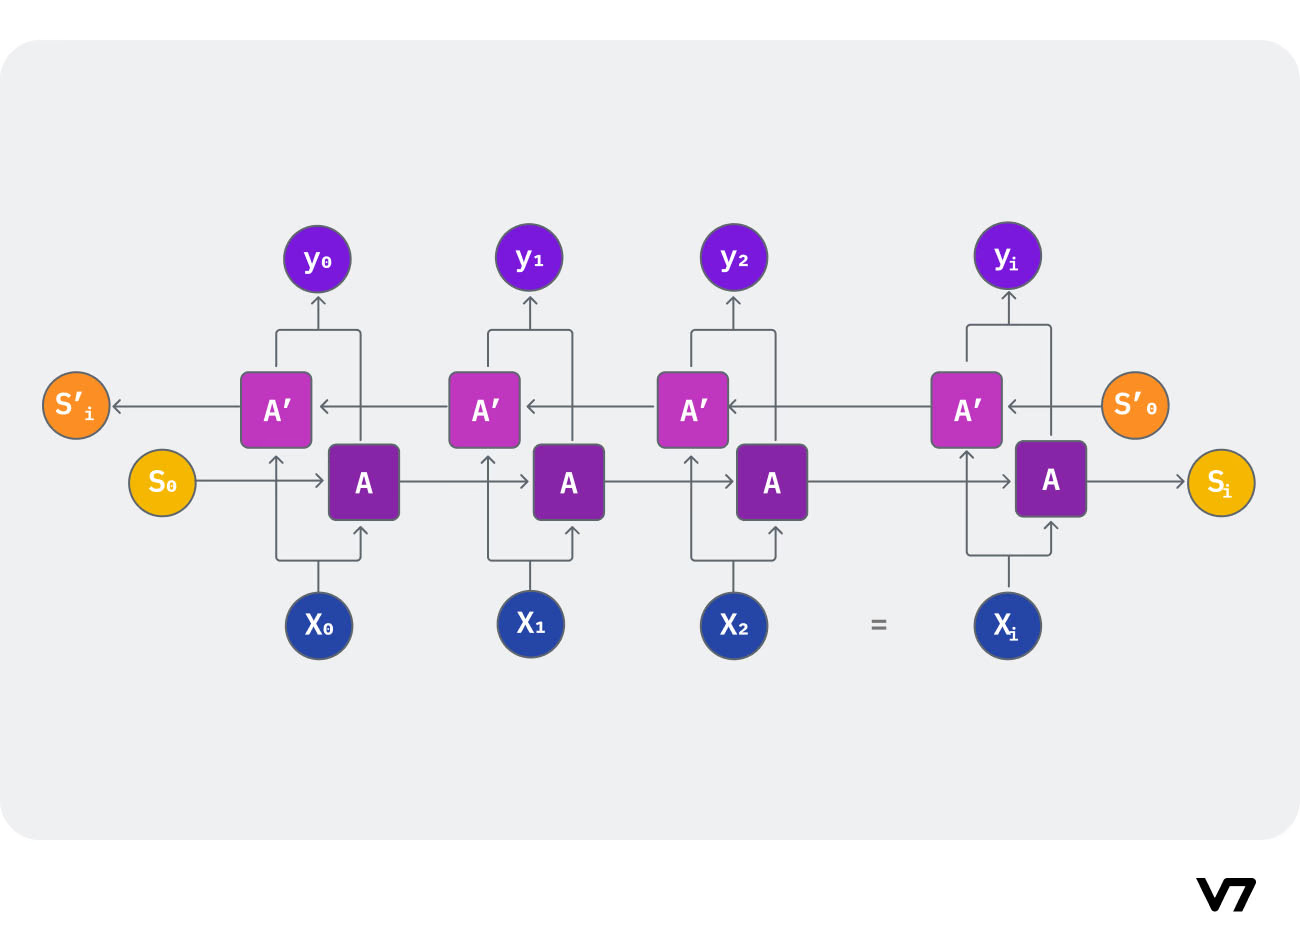
\includegraphics[scale=0.25]{brnn.png}
    \caption{Red Neuronal Recurrente Bidireccional.}
\end{figure}

\newpage

\subsubsection{Memoria a corto y largo plazo (LSTM)}
LSTM es una arquitectura RNN popular, que fue introducida por Sepp Hochreiter y Juergen Schmidhuber como una solución al problema del gradiente evanescente. En su artículo \cite{lstmpaper} trabajan para abordar el problema de las dependencias a largo plazo. Es decir, si el estado anterior que influye en la predicción actual no se encuentra en el pasado reciente, es posible que el modelo RNN no pueda predecir con exactitud el estado actual. \\

Por ejemplo, supongamos que queremos predecir las palabras en cursiva que siguen: ``Alicia es alérgica a los frutos secos. No puede comer mantequilla de cacahuete''. El contexto de una alergia a los frutos secos puede ayudarnos a anticipar que los alimentos que no se pueden comer contienen frutos secos. Sin embargo, si ese contexto estuviera unas frases antes, dificultaría, o incluso imposibilitaría, que la RNN conectara la información. \\

Para solucionarlo, las LSTM tienen ``celdas'' en las capas ocultas de la red neuronal, que tienen tres puertas: una puerta de entrada, una puerta de salida y una puerta de olvido. Estas puertas controlan el flujo de información que se necesita para predecir la salida en la red. Por ejemplo, si los pronombres de género, como ``ella'', se repitieron varias veces en oraciones anteriores, puede excluirlos del estado de la celda. \\

\begin{figure}[H]
    \centering
    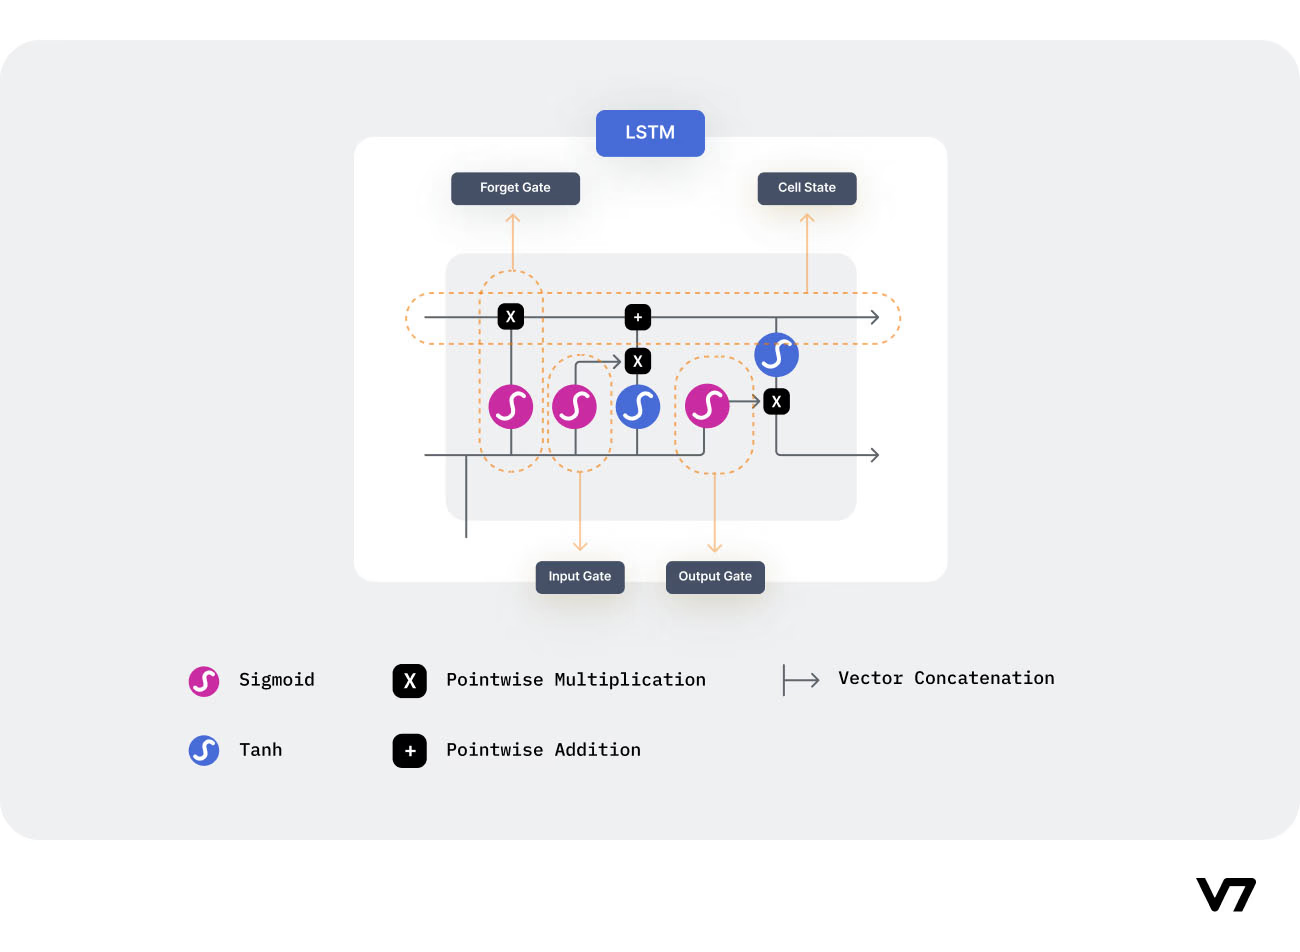
\includegraphics[scale=0.3]{lstm.png}
    \caption{Memoria a Corto y Largo Plazo.}
\end{figure}

\newpage

\subsubsection{Unidades recurrentes bloqueadas (GRU)}
Pueden darse escenarios en los que aprender únicamente de los datos inmediatamente anteriores en una secuencia sea insuficiente. Consideremos el caso de intentar predecir una frase basada en otra frase introducida mucho antes en un libro o artículo. En este caso, recordar tanto los datos inmediatamente precedentes como los anteriores resulta crucial. Una RNN, debido a su mecanismo de compartición de parámetros, utiliza los mismos pesos en cada paso de tiempo. Como resultado, la retropropagación puede hacer que el gradiente explote o se desvanezca, y la red neuronal no aprende mucho de los datos que están alejados de la posición actual. \\

Las GRU utilizan dos puertas: la puerta de actualización (update gate) y la puerta de reinicio (reset gate). Básicamente, estas son dos vectores que deciden qué información debe pasarse a la salida. Lo especial de estas puertas es que pueden entrenarse para conservar información a largo plazo sin degradarla con el tiempo o para eliminar información irrelevante para la predicción.

\begin{itemize}
    \item \textbf{Puerta de actualización}: es responsable de determinar la cantidad de información previa que debe pasar al siguiente estado.
    \item \textbf{Puerta de reinicio}: se usa para decir cuánta información del pasado debe ser ignorada por el modelo.
\end{itemize}

\begin{figure}[H]
    \centering
    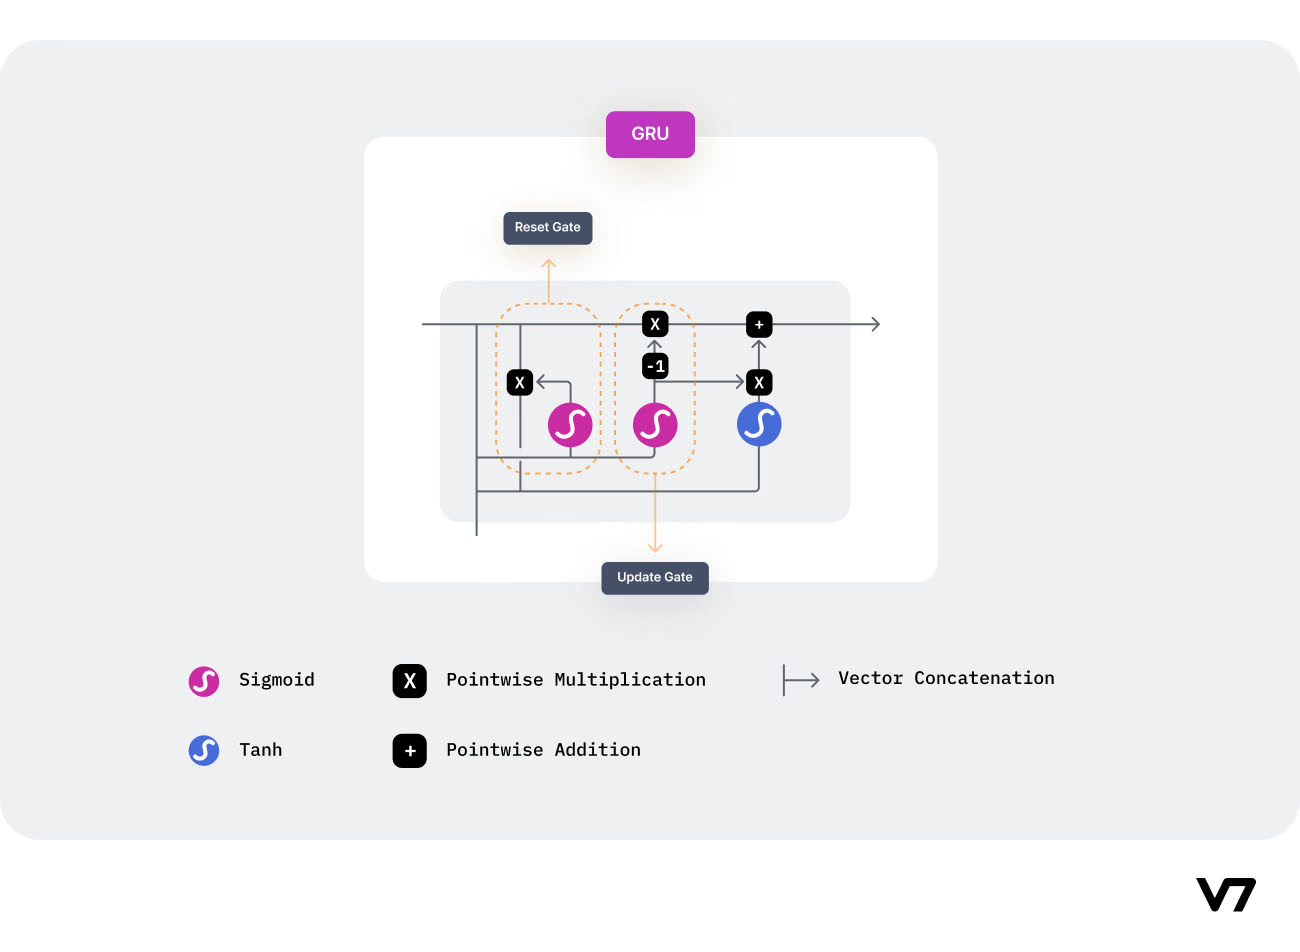
\includegraphics[scale=0.3]{gru.png}
    \caption{Unidades Recurrentes Bloqueadas.}
\end{figure}

\newpage

\subsection{Desafíos de las RNN estándar}
Entrenar una RNN, o cualquier red neuronal, se realiza definiendo una función de pérdida que mide el error o la desviación entre el valor predicho y la verdad fundamental (\textbf{ground truth}). Las características de entrada se procesan a través de múltiples capas ocultas que utilizan diferentes o las mismas funciones de activación, y se predice el resultado. La función de pérdida total se calcula, marcando así el final de la \textit{pasada hacia adelante} (\textbf{forward pass}). \\

La segunda parte del entrenamiento es la \textit{pasada hacia} atrás (\textbf{backward pass}), donde se calculan las diversas derivadas. Este proceso se vuelve aún más complejo en las Redes Neuronales Recurrentes (RNN), ya que estas procesan datos secuenciales o dependientes del tiempo. El modelo debe retropropagar los gradientes no solo a través de todas las capas ocultas, sino también a través del tiempo. Por lo tanto, en cada paso de tiempo, tiene que sumar todas las contribuciones anteriores hasta el instante de tiempo actual. \\

\begin{itemize}
    \item \textbf{Gradientes Explosivos}: En algunos casos, los valores de los gradientes continúan aumentando hasta alcanzar el infinito de forma exponencialmente rápida. Esto provoca actualizaciones de pesos muy grandes y hace que el descenso de gradiente diverja, volviendo el proceso de entrenamiento extremadamente inestable. Este problema se conoce como el gradiente explosivo (exploding gradient).
    \item \textbf{Gradientes desvanecidos}: En otros casos, a medida que la retropropagación avanza desde la capa de salida hacia la capa de entrada, el término del gradiente tiende a cero de forma exponencialmente rápida. Como resultado, los pesos de las capas iniciales o más profundas apenas cambian, lo que dificulta que el modelo aprenda dependencias de largo plazo. Esto provoca que el descenso de gradiente nunca converja al óptimo. Este problema se conoce como el gradiente desvanecido (vanishing gradient).
\end{itemize}

\newpage
\subsection{Generación de Texto}
\subsubsection{Definición del problema}
\subsubsection{Flujo del modelo: tokenización, embeddings, RNN, decodificación}
\subsubsection{Métricas para evaluar el texto generado}

\subsection{Comparación con otros enfoques}
\subsubsection{RNN vs Transformers}

\subsection{Ventajas y Desventajas de las RNN}
\subsection{Problemas de las RNN}
\subsection{Aplicaciones de las RNN}
\subsubsection{Procesamiento del Lenguaje Natural (NLP)}
\subsubsection{Series Temporales}
\subsubsection{Reconocimiento de Voz}

\newpage

\section{Implementación Práctica}
\subsection{Preparación de Datos}
\subsubsection{Descarga y preprocesamiento del texto}
\subsubsection{Tokenización y codificación}
\subsubsection{Generación de ventanas (ventanas deslizantes)}

\subsection{Arquitectura del Modelo}
\subsubsection{Detalles de la arquitectura \texttt{CharRNN}: embeddings, LSTM, capa de salida}
\subsubsection{Hiperparámetros del modelo}
\subsubsection{Visualización de la arquitectura (diagrama opcional)}

\subsection{Entrenamiento}
\subsubsection{Configuración del entrenamiento (batch size, epochs, optimizador)}
\subsubsection{Función de pérdida y retropropagación}
\subsubsection{Monitoreo de métricas (pérdida de entrenamiento y validación)}

\subsection{Generación de Texto}
\subsubsection{Proceso de inferencia}
\subsubsection{Ajuste de la temperatura para variar la creatividad del texto generado}
\subsubsection{Ejemplos de texto generado}

\addtocontents{toc}{\protect\newpage}

\section{Resultados}
\subsection{Pérdida de entrenamiento y validación (gráficos de convergencia)}
\subsection{Ejemplos de texto generado}
\subsubsection{Texto inicial (épocas tempranas)}
\subsubsection{Texto final (épocas avanzadas)}
\subsection{Comparación con el estilo literario original (\textit{Don Quijote})}
\subsection{Observaciones sobre la coherencia del texto generado}

\newpage

\section{Conclusiones}
\subsection{Resumen de los resultados obtenidos}
\subsection{Fortalezas y limitaciones del modelo}
\subsection{Propuestas de mejora}
\subsubsection{Experimentar con GRU/LSTM más profundas}
\subsubsection{Uso de Transformers o más datos}

\section{Anexos}
\subsection{Código completo del proyecto (o enlace a un repositorio)}
\subsection{Explicación de cómo instalar y ejecutar el proyecto}
\subsubsection{Dependencias necesarias (PyTorch, tqdm, etc.)}
\subsubsection{Instrucciones para reproducir los resultados}
\subsection{Documentación adicional sobre métricas y técnicas utilizadas}

\newpage

\section{Bibliografía}
\nocite{*}
\printbibliography

\end{document}